\chapter{Nested and Subpattern Yielding}%\chapter{Declarative and Imperative Pattern Parts}
\indexmain{yielding}\label{cha:yielding}

In this chapter we explain an extension of the LHS and RHS patterns by yielding parts.
The constructs seen so far are executed top-down alongside the contained nested and subpatterns, for one during matching and for the other during rewriting.
The yielding parts are executed bottom-up for one after matching and for the other while rewriting, they allow to accumulate results.
Syntactically, the split is denoted by a separator line \texttt{---}.
The content before the split is mostly related to declarative pattern matching and rewriting (following the idea of graph rewriting), while the content after the split supplements them by more powerful imperative features.

\begin{table}[htbp]
  \centering
  \begin{tabularx}{\linewidth}{|l|X|X|} 
		\hline
     & top-down (declarative) & bottom-up (imperative extensions) \\
		\hline
    LHS pattern & pattern matching & result accumulation \\
		\hline
    RHS pattern & rewriting & result accumulation (computations) \\
		\hline
  \end{tabularx}
  \caption{Pattern separator}
  \label{patternsepar}
\end{table}

As a refinement regarding the execution semantics:
we have two runs, the first matching run constructs a match object tree (reflecting the LHS pattern parts and their nesting structure),
the second run walks the match object tree and carries out rewriting alongside it.
After the rewriting run are the embedded execs executed (they get encapsulated and stored in closures during the walk, the top-level ones are executed directly).

The match objects consist of the pattern elements bound by top-down pattern matching,
and of new LHS def elements that receive the data from bottom-up yielding
(these amount to inherited and synthesized attributes in compiler construction parlance).

%TODO: integrate
% (or iterated matches accumulation shortcuts)
%local pattern elements/graphlet vs nested/subpattern.
%So data flows first top-down and then bottom-up during nested/subpattern processing (for the LHS strictly separated (IAG and SAG), for the RHS the user may choose an order of match attribute evaluation/nested object visiting (LAG with self-defined L)).
%TODO: tell explicitly?:
% - on LHS appear to the left of the separator the elementary pattern entities, nested patterns, and subpattern usages, and to the right of the separator the def elements and yield blocks
%   (in subpattern usages, the input and output arguments are separated by the ---, too, the same holds for the %input and output parameters in the subpattern specifications)
%   (the return (in tests) has to come right of the separator in case that one is given)
% - on RHS appear to the left of the separator the pattern rewrite specifications and attribute changing eval blocks, and to the right of the separator the def elements, eval blocks supporting all computations, emit and exec statements, as well as the ordered statements (telling when the rewrite which nested/subpattern, emithere, evalhere)
%   (in subpattern usages, the rewrite input and output arguments are separated by the ---, too, the same holds for the rewrite input and output parameters in the subpattern specifications)
%   (the return (in rules) has to come right of the separator in case that on is given)

\section{Yielding Outwards After Pattern Matching} 

Sometimes one needs to bring something matched within a nested or subpattern to an outer pattern containing it (nested patterns) or calling it (subpatterns).
So one can return it out, or accumulate information from matched iterated pattern instances. 

\subsection{LHS def variables} 

\begin{rail} 
  LHSPatternDefVariableDecl: 
	('def' IdentDecl ':' Type |
	'def' '-' IdentDecl ':' Type '->' |
	'def' 'var' IdentDecl ':' Type |
	'def' 'ref' IdentDecl ':' Type ) \\
	('=' Expression)? ('=' YieldExpression)? ';'
	;
\end{rail}\ixnterm{DefVariableDecl}

The first thing one needs to bring something outwards is a target in a nesting or calling pattern. 
This is achieved by nodes, edges, and variables declared with the \texttt{def} keyword in the pattern, marking them as output entities.
Furthermore subpattern parameters may be declared as def parameters in the subpattern definition header,
marking them as output parameters.

\subsection{Yielding and Iterated Filtering} 

\subsubsection*{Yield blocks} 

These elements can then be yielded to by \texttt{eval} statements from within a \texttt{yield} block
(maybe with iterated accumulation) and subpattern usages.
A \texttt{yield} block is a constrained \texttt{eval} block that can be given in the pattern part;
it does not allow to assign to or change non-\texttt{def} variables, or carry out graph-changing commands.
Yielding is specified by prepending the \texttt{yield}\indexmain{yield} keyword to the entity yielded to,
in the assignment or method call.
The \texttt{yield} must be prepended to the argument for a subpattern def parameter, too.

Yielding, i.e. bubbling up of the elements in the match object tree occurs at the end of pattern matching when the match object tree gets constructed.

%warning evt only in RHS part
\begin{warning}
A def entity from the pattern part can't be yielded to from the rewrite part, they are constant after matching.
\end{warning}

Let's have a look at two examples for yielding:

\begin{example}
  \begin{grgen}
pattern Chain(begin:Node --- def end:Node)
{
  alternative {
    further {
      begin --> next:Node;
      :Chain(next --- yield end);
    }
    done {
      negative {
        begin --> ;
      }
      ---
      yield {
        yield end = begin;
      }
    }
  }
}
pattern LinkChainTo(begin:Node) modify(n:Node)
{
  alternative {
    further {
      begin --> next:Node;
      o:LinkChainTo(next);

      modify {
        next --> n;
        o(n);
      }
    }
    done {
      negative {
        begin --> ;
      }

      modify {
      }
    }
  }

  modify { }
}
rule linkChainEndToStartIndependent(begin:Node) : (Node)
{	
  independent {
    c:Chain(begin --- yield end);
  }
  o:LinkChainTo(begin);
--- 
  def end:Node;

  modify {
    o(end);
    return(end);
  }
}
  \end{grgen}
\end{example}

The first example for LHS yielding follows within an independent a chain piece by piece to some a priori unknown end node, and yields this end node chain piece by chain piece again outwards to the chain start. There it is used as input to another chain (maybe the same chain, maybe overlapping due to the independent), linking all the nodes of this chain to the end node of the former.

When yielding from an iterated pattern there's the issue that a simple bottom-up assignment to a def variable from the outside would only overwrite the variable value multiple times, so we would end up with one of the values from the iterated pattern instances (indeterministically chosen -- multiple iterated variable values exist for a single nesting pattern variable).
But we can also read entities from the nesting pattern, and thus use them as accumulation variables, for e.g. summing integers or concatenating strings.
The start value of accumulation can be set with the initialization in the nesting pattern (and thus travels top-down).

\begin{example}
  \begin{grgen}
test sumOfWeight(start:Node) : (int,int)
{
  iterated {
    start --> n:N; // node class N { a:int; }
  ---
    yield {
      yield sum = sum + n.a;
      yield v = n.a; // v is in the end the n.a of one iterated instance
    }
  } 
---
  def var sum:int = 0;
  def var v:int = 0;
  return (sum,v);
}
  \end{grgen}
\end{example}

Alternatively, a \texttt{for} iterated accumulation loop can be used, iterating a def variable inside an iterated for all the matches of the iterated pattern referenced by name, it allows to assign to an outside def variable a value computed from the def variable and the value of the iterated def variable.

This is shown in the third example for LHS yielding, summing the integer attribute \texttt{a} of nodes of type \texttt{N} adjacent to a start node, matched with an iterated.

\begin{example}
  \begin{grgen}
test sumOfWeight(start:Node) : (int)
{
  iterated it {
    start --> n:N; // node class N { a:int; }
  ---
    def var i:int = n.a;
  } 
---
  def var sum:int = 0;
  yield {
    for(i in it)
    {
      yield sum = sum + i;
    }
  }

  return (sum);
}
  \end{grgen}
\end{example}

In case no accumulation is needed but a simple \indexed{count} of the iterated matches is sufficient, one can employ the \texttt{count} operator on an iterated (that must have been named before), as displayed in the following example (the count is only available in a \texttt{yield} or \texttt{eval} block).

\begin{example}
  \begin{grgen}
test countOfEdges(start:Node) : (int)
{
	iterated it {
		start -->;
	} 
---
	def var sum:int = 0;
	yield {
		yield sum = count(it);
	}

	return (sum);
}
  \end{grgen}
\end{example}

\subsubsection*{Yield expressions} 

\begin{rail} 
  YieldExpression: 'yield' '(' Expression ')' ;
\end{rail}\ixnterm{YieldExpression}\ixkeyw{yield}

For more convenience, the notational shorthand of in-place yielding at a def variable declaration is available.
The syntactic sugar with the syntax \texttt{def var v:T = yield(expr);} is de-sugared to a plain \texttt{def var v:T;} declaration and an assignment in an implicitly added \verb#yield { v = expr; }# block.
It is not to be confused with separate initialization, combined: \texttt{def var v:T = init-expr = yields(expr)} --- the init-expr is evaluated before the yields of nested patterns and can thus be used to give a start value for bottom-up accumulation, the in-place yielding is evaluated after nested and subpatterns were matched and yielded (only then are iterated matches available).

The example from above can be formulated succintly with the yield expression.

\begin{example}
  \begin{grgen}
test countOfEdges(start:Node) : (int)
{
	iterated it {
		start -->;
	} 
---
	def var sum:int = yield(count(it));
	return (sum);
}
  \end{grgen}
\end{example}


A more general language device that benefits from the yield expression is the \indexed{iterated query}. 
It is available in the rule language expressions within a rule (but only during yielding), and returns an array of the matches of the iterated (\texttt{array<match<r.it>>} for iterated \texttt{it} in rule \texttt{r}), cf. Section~\ref{sec:primexpr}, in contrast to the rule query from Chapter~\ref{cha:graphquery} that is available in the sequence expressions, and returns an array of matches of the rule (\texttt{array<match<r>>}).
Similar to the \texttt{for} iterated accumulation loop, it accesses the matches of the iterated from the outside (in contrast to default bottom-up yielding from inside).
Employing the iterated query, the example looks as follows; for a larger example, see Example~\ref{exsimplequeryrules}.

\begin{example}
  \begin{grgen}
test countOfEdges(start:Node) : (int)
{
	iterated it {
		start -->;
	} 
---
	def var sum:int = yield([?it].size());
	return (sum);
}
  \end{grgen}
\end{example}
	
	
\subsubsection*{Iterated Filtering}\label{sub:iteratedfilter}

A helper in iterated accumulation is iterated filtering, it allows to execute filters on the iterated matches array, reordering matches or even removing them (thus changing the result matches tree of rule application).
For this to work, the iterated must be firstly given a name, as described in \ref{namednested}, so it can be referenced, and secondly, a filter must be declared on it, cf. Section~\label{cardinality} (unless only auto-supplied filters are to be applied, cf. \ref{filter:auto-supplied}).

\begin{rail}
  IteratedFiltering: 
    'iterated' IteratedIdent FilterCalls ';';
\end{rail}\ixkeyw{IteratedFiltering}

The syntax of the iterated filtering specification past the \texttt{iterated} \emph{IteratedIdent} part is the same as for filter calls on a rule, e.g. \verb#r\f#, see Chapter~\ref{sub:filters} for more on this.
Note that the feature is limited to top-level iterateds for now.

\begin{example}
  \begin{grgen}
test iteratedFiltering(start:Node) : (int)
{
	iterated it {
		start --> n:N;
	---
		def var i:int = n.i;
	} 
---
	iterated it \ orderDescendingBy<i> \ keepFirst(3);
	def var sum:int = yield([?it].extract<i>().sum());
	return (sum);
}
  \end{grgen}
\end{example}


\pagebreak

%%%%%%%%%%%%%%%%%%%%%%%%%%%%%%%%%%%%%%%%%%%%%%%%%%%%%%%%%%%%%%%%%%%%%%%%%%%%%%%%%%%%%%%%%%%%%%%%

\section{Yielding Outwards During Rewriting} \label{sec:localvarorderedevalyield}\indexmain{local variable}\indexmain{evalhere}\indexmain{yielding outwards}

Sometimes one needs to bring something obtained during rewriting within a nested or subpattern to an outer pattern containing it (nested patterns) or calling it (subpatterns).
So that one can do there (in the using pattern) operations on it, e.g. attaching a further edge to an end node of a chain matched with recursive patterns (thus modularizing the graph rewrite specification into chain matching patterns and patterns using chains doing things on the chain ends), or accumulating attributes obtained in iterated pattern instances. 

\subsection{RHS def variables} 

The first thing one needs to bring something outwards is a target in a nesting or calling pattern. 
This is achieved by nodes, edges, and variables declared with the \texttt{def}\indexmain{def} keyword in a rewrite part, marking them as output entities.
%variables were already introduced in previous paragraphs, but in addition to them nodes and edges are allowed, too.
In addition, on their introduction an initializing expression may be given.
Furthermore subpattern rewrite parameters may be declared as def parameters,
marking them as output parameters.

\begin{rail} 
  RHSPatternDefVariableDecl: 
	('def' IdentDecl ':' Type |
	'def' '-' IdentDecl ':' Type '->' |
	'def' 'var' IdentDecl ':' Type |
	'def' 'ref' IdentDecl ':' Type ) \\
	('=' Expression)? ';'
	;
\end{rail}\ixnterm{RHSPatternDefVariableDecl}

Another use besides bringing something upwards/to the outside is as a helper in attribute evaluation,
as temporary variables (but local variables introduced in the computation are preferable in case they are only used in their very computation).
%Such local variables can be introduced on a right hand side employing the known variable syntax \texttt{var name:type}, prefixed with the \texttt{def} keyword.
%From then on they can be read and be assigned to in \texttt{evalhere} statements of the RHS, or used as variable parameters in subpattern rewrite calls.

\begin{example}
  \begin{grgen}
rule r : (double) {
  n1:N; n2:N; n3:N;
  
  modify {
  ---
    def var mean:double = array<double>(n1.v, n2.v, n3.v).avg();
    eval {
      n1.variance = Math::sqr(n1.v - mean); 
      n2.variance = Math::sqr(n2.v - mean); 
      n3.variance = Math::sqr(n3.v - mean); 
    }
    return(mean);
  }
}
  \end{grgen}
\end{example}

\subsection{Yielding}\label{sub:yield} 

These elements can then be yielded to from within \texttt{eval} or \texttt{evalhere} statements, subpattern rewrite usages, or \texttt{exec} statements.
While the latter will be covered in chapter \ref{cha:imperativeandstate}, the former will be explained in the following.

Yielding is specified by prepending the \texttt{yield}\indexmain{yield} keyword to the entity yielded to,
in an assignment or a change assignment to a variable, or a method call on a variable,
inside an \texttt{eval} or \texttt{evalhere}-block; 
the target of the assignment may be a node or edge (if declared as output variable).
The yield must be prepended to the argument for a subpattern def rewrite parameter, too.

\begin{example}
  \begin{grgen}
pattern Chain(begin:Node) modify(--- def end:Node)
{
  alternative {
    Further {
      begin --> intermediate:Node;
      c:Chain(intermediate);
      
      modify {
        c(--- yield end);
      }
    }
    Done {
      negative {
        begin --> ;
      }
      
      modify {
      ---
        eval {
          yield end = begin;
        }
      }
    }
  }
  
  modify { }
}

rule R(begin:Node) : (Node) {
  c:Chain(begin);

  modify {
    c(--- yield end); // end is filled with chain end
  ---
    def end:Node;
    return(end);
  }
}
  \end{grgen}
  First example for RHS yielding: returning the end node of a chain.
\end{example}

\begin{example}
  \begin{grgen}
rule outCount(head:Node) : (int)
{
  iterated {
    head --> .;
    modify {
    ---
      eval { yield cnt = cnt + 1; }
    }
  }

  modify {
  ---
    def var cnt:int = 0;
    return (cnt);
  }
}
  \end{grgen}
  Second example for RHS yielding: counting the number of edges matched with an iterated.
\end{example}

%\pagebreak


%%%%%%%%%%%%%%%%%%%%%%%%%%%%%%%%%%%%%%%%%%%%%%%%%%%%%%%%%%%%%%%%%%%%%%%%%%%%%%%%%%%%%%%%%%%%%%%%
\section{Flow Example}\label{matchingflow}

Pattern matching and rewriting occurs in two completely distinct passes, separated by the matches tree of the sub- and nested patterns.
During each pass, input and output parameters may be computed and passed; with explicit passing for subpatterns, and implicit passing for nested patterns (which can directly access the content of their contained pattern).

First the pattern is matched with recursive descent alongside pattern nesting and subpattern calling, employing some helper stacks in addition to the call stack (the pushdown machine is explained in more detail in \ref{sec:generatedcode}).
Matching occurs strictly top-down (or from the outside to the nested inside patterns), first the graphlets of the current pattern are matched, then control descends to the nested and subpatterns.
During matching, input parameters may be passed, esp. forwarding just matched elements or attributes from them; they allow to influence the matching process.

When a complete match is found, while ascending again, unwinding the call stack, output pattern-\texttt{def} parameters are passed bottom-up (or from the inside to the containing outside patterns) with \texttt{yield} blocks and \texttt{yield} assignments within those blocks, or \texttt{yield} bindings of \texttt{def} parameters in a subpattern call.
During this ascent, the matches tree is assembled, each match of a pattern contains the matches of its nested patterns and used subpatterns when it is left.

In the rewrite step, the matches tree is visited recursively again, creating the new nodes of the current pattern, then descending to the nested patterns and subpatterns, executing their changes, and after they returned, executing all other changes of the pattern.
During this visit, rewrite input parameters may be passed, for forwarding just created elements (or computed values). 

On ascending again from a pattern, the rewrite-\texttt{def} elements are assigned from \texttt{yield} assignments in the \texttt{eval} blocks, or \texttt{yield} bindings of \texttt{def} rewrite parameters in a subpattern rewrite call.
(Technically, nested patterns are handled like subpatterns, with parameter passing for accessed elements of the containing pattern automatically inserted by the compiler.)

Let's take a look at an example, with Figure \ref{figmatchingparameterflow} depicting the input and output parameter passing during the matching of Example \ref{exmatchingparameterflow}, and Figure \ref{figrewritingparameterflow} depicting the input and output parameter passing during the rewriting of Example \ref{exrewritingparameterflow} (which is an extended version of Example \ref{figmatchingparameterflow}).

\begin{example}
  \begin{grgen}
rule r(a:Node) : (Node, int)
{
  a --> b:Node;
  p:P(b --- yield d);

  optional o {
    a --> . --> c:N;
  ---
    yield { yield i = c.i; }

    modify {
    }
  }
---	
  def var i:int;
  def d:Node;

  modify {
    b --> u:Node;
    return(d, i);
  }
}
pattern P(n:Node --- def rm:Node)
{
  n --> . --> m:Node;
---
  yield { yield rm = m; }
}
  \end{grgen}
\end{example}\label{exmatchingparameterflow}

\begin{figure}[hptb]
  \centering
  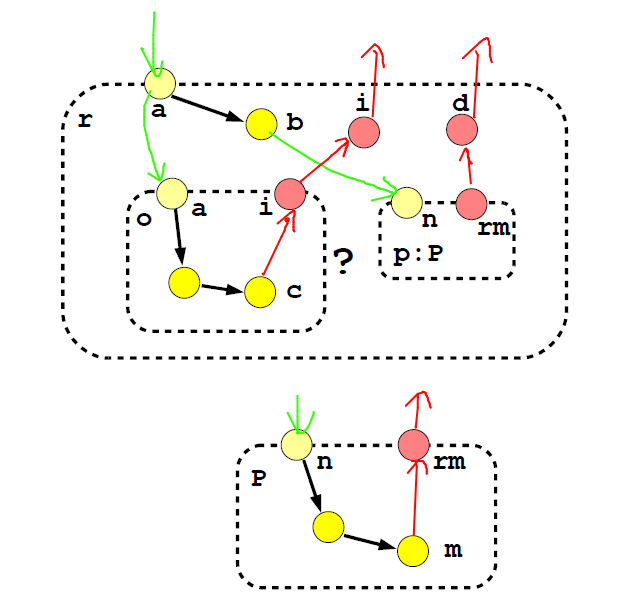
\includegraphics[width=0.61\textwidth]{fig/MatchAndParameterFlowAnnotated}
  \caption{Parameter flow in matching}
  \label{figmatchingparameterflow}
\end{figure}

\begin{example}
  \begin{grgen}
rule r(a:Node) : (Node, int, Node, int) {
  a --> b:Node;
  optional o {
    a --> . --> c:N;
  ---
    yield {	yield i = c.i; }

    modify {
    ---
      eval { yield j = i + u.i; }
    }
  }
  p:P(b --- yield d);
---	
  def var i:int;
  def d:Node;

  modify {
    b --> u:N;
    p(u --- yield e);
  ---
    def e:Node; def var j:int;
    return(d, i, e, j);
  }
}
pattern P(n:Node --- def rm:Node) modify(k:Node --- def x:Node) {
  n --> . --> m:Node;
---
  yield {	yield rm = m; }

  modify {
    m --> k; m --> l:Node;
  ---
    eval { yield x = l; }
  }
}
  \end{grgen}
\end{example}\label{exrewritingparameterflow}

\begin{figure}[hptb]
  \centering
  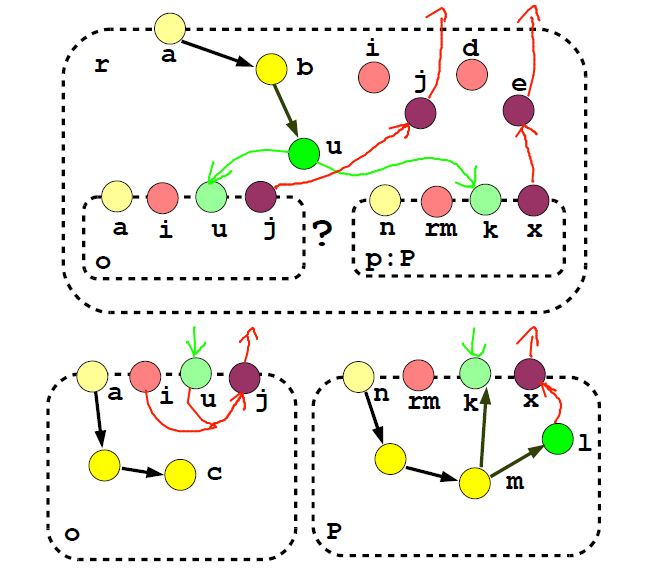
\includegraphics[width=0.63\textwidth]{fig/RewriteAndParameterFlowAnnotated}
  \caption{Parameter flow in rewriting}
  \label{figrewritingparameterflow}
\end{figure}

In Example \ref{exmatchingparameterflow}, a rule \texttt{r} is matched, which contains a nested \texttt{optional} pattern \texttt{o} and uses a subpattern \texttt{P}.
The rule matches from its input node \texttt{a} on a neighbouring node \texttt{b} and hands it in to the subpattern \texttt{p}.
In the optional pattern it matches a two-step neighbouring node \texttt{c} from \texttt{a} on.
The subpattern \texttt{P} matches from its input parameter \texttt{n} on a two-step neighbouring node \texttt{m}.

A \texttt{def} variable \texttt{i} is declared in the pattern, and \texttt{yield} assigned from the optional \texttt{o} an attribute of the \texttt{c} found there.
Another \texttt{def} variable \texttt{d} is declared in the pattern, and assigned from the subpattern call \texttt{p} with a \texttt{yield} parameter passing. 
The two pattern \texttt{def} variables are then \texttt{return}ed out of rule \texttt{r}.
The subpattern \texttt{P} \texttt{yield}s to its output \texttt{def} parameter \texttt{rm} the \texttt{m} found in its body.

In the extended Example \ref{exrewritingparameterflow}, the rewrite part of the rule \texttt{r} creates a node \texttt{u}, links it to \texttt{b}, and hands it in to the subpattern rewrite employment of \texttt{p}.
The rewrite part of subpattern \texttt{P} creates a node \texttt{l} and links it to \texttt{m}.
Additionally, an edge is inserted in between \texttt{m} and the rewrite input parameter \texttt{k}.

A \texttt{def} variable \texttt{j} is declared in the rewrite part of \texttt{r}, and \texttt{yield} assigned from the \texttt{eval} inside the rewrite part of the optional \texttt{o}.
Another \texttt{def} variable \texttt{e} is declared in the rewrite part, and assigned from the subpattern rewrite call \texttt{p}.
The two rewrite-\texttt{def} variables are then \texttt{return}ed out of the rule, in addition to the two pattern-\texttt{def} variables.
The subpattern \texttt{yield}s from its \texttt{eval} part to its output \texttt{def} rewrite parameter \texttt{x} the \texttt{l} just created.

Bottom line: you can flexibly combine patterns with nested and subpatterns, including input and output parameters.
You can pass parameters in during matching alongside matching order. When matching completed, during match-tree building, you can yield elements found in contained patterns out. 
When the rewrite is applied, you can pass parameters in alongside the buildup of the patterns, and yield elements out once more.
But not only are those two passes strictly distinct, but also are the parameter passing directions strictly distinct, first is all input parameter passing carried out during descent, then is all output parameter synthesizing carried out during ascent.


%%%%%%%%%%%%%%%%%%%%%%%%%%%%%%%%%%%%%%%%%%%%%%%%%%%%%%%%%%%%%%%%%%%%%%%%%%%%%%%%%%%%%%%%%%%%%%%%
\section{Ordered Evaluation} \label{sec:localvarorderedevalyield}\indexmainsee{evalhere}{ordered evaluation}

Normally the rewrite order is as given in table \ref{table:executionorderrewriting}:
\begin{table}[htbp]
  \centering
  \begin{tabularx}{\linewidth}{|l|X|} \hline
    \texttt{ 1. } & \texttt{ Extract elements needed from match } \\
    \texttt{ 2. } & \texttt{ Create new nodes } \\
    \texttt{ 3. } & \texttt{ Call rewrite code of used subpatterns} \emph{and more...} \\ 
	  \texttt{ 4. } & \texttt{ Call rewrite code of nested iterateds } \\
    \texttt{ 5. } & \texttt{ Call rewrite code of nested alternatives } \\
    \texttt{ 6. } & \texttt{ Redirect edges } \\  
    \texttt{ 7. } & \texttt{ Retype (and merge) nodes } \\  
    \texttt{ 8. } & \texttt{ Create new edges } \\
    \texttt{ 9. } & \texttt{ Retype edges } \\  
    \texttt{ 10. } & \texttt{ Create subpatterns } \\
    \texttt{ 11. } & \texttt{ Attribute reevaluation (eval) } \\
    \texttt{ 12. } & \texttt{ Remove edges } \\ 
	  \texttt{ 13. } & \texttt{ Remove nodes } \\
    \texttt{ 14. } & \texttt{ Remove subpatterns } \\
    \texttt{ 15. } & \texttt{ Emit / Exec } \\  
    \texttt{ 16. } & \texttt{ Return } \\ \hline
	\end{tabularx}
	{\small \emph{and more...} at \texttt{3.} are \texttt{evalhere}, \texttt{emithere}, \texttt{emitheredebug}, \texttt{alternative} Name, \texttt{iterated} Name}
  \caption{Execution order rewriting}
  \label{table:executionorderrewriting}
\end{table}

So first the subpatterns rewrites, then the iterated rewrites, then the alternative rewrites are executed, and finally the local eval statements (computations).
This might be sufficient in some cases, but in other cases, e.g. when you want to compute an attributation over a tree/a graph, you want to have local computations influenced by attributes in nested/called children or its siblings, and attributes in nested/called children influenced by its parents or siblings.
So we need a language device which allows us to specify the execution order of the alternative pattern rewrites versus the iterated pattern rewrites versus the subpattern rewrites versus the local attribute evaluations.

To achieve attribute evaluation or pattern rewriting in a defined order, we use order specifications.
They get executed in the order in which they are given syntactically,
in the form of \emph{CardinalityRewriteOrderSpecification}s and \emph{AlternativeRewriteOrderSpecification}s for nested patterns,
in the form of \emph{SubpatternRewriteOrderSpecification}s for subpatterns,
and in the form of local attribute evaluations in \texttt{evalhere} blocks;
a further statement executed in order is \texttt{emithere}, introduced in \ref{sec:deferredexecemithere}. 

\begin{rail}  
  CardinalityRewriteOrderSpecification: 
    ('iterated' | 'multiple' | 'optional') Ident ';';
  AlternativeRewriteOrderSpecification: 
    'alternative' Ident ';';
  SubpatternRewriteOrderSpecification: 
    'pattern' Ident ';';
\end{rail}

The \emph{CardinalityRewriteOrderSpecification} and \emph{AlternativeRewriteOrderSpecification} reference the iterated or alternative by its name, so a name must be defined, cf. \ref{namednested}.
So does the \emph{SubpatternRewriteOrderSpecification}, which is not to be confused with the \emph{SubpatternRewriteApplication} introduced in \label{sec:subrule}, the latter only specifies that the subpattern is to be rewritten (disregarding order), additionally giving the rewrite arguments.

What we've seen so far is applied in the following example.
A \texttt{yield} prefix is needed whenever a \texttt{def} variable from a level above is written to (as assignment target as well as a subpattern output argument). 

\begin{example}
  \begin{grgen}
rule R {
  iterated foo { .; modify { ..read i.. } }
  alternative bar { case { modify { ..read i.. } } } 
  sub1:Subpattern1();
  sub2:Subpattern2();

  modify {
    sub1(i);
    sub2(i);
  ---
    def var i:int = 0; // initializes i to 0
    evalhere { yield i = i + 1; } // afterwards i==1
    pattern sub1; // input 1 to subpattern rewrite
    evalhere { yield i = i + 1; } // afterwards i==2
    iterated foo; // nested iterated reads i==2 
    evalhere { yield i = i + 1; } // afterwards i==3
    alternative bar; // nested alternative reads i==3
    evalhere { yield i = i + 1; } // afterwards i==4
    pattern sub2; // input 4 to subpattern rewrite
    evalhere { yield i = i + 1; } // afterwards i==5
    eval { yield j = i + 1; } // assign 6 to j
  }
}
  \end{grgen}
\end{example}

\begin{note}
For rewriting, the execution order of the parts can be defined, to allow programming attribute evaluation orders of interest, defining when to descend into which part and defining glueing/local computations in between.
(A depth first run with a defined order in between the siblings, comparable to an LAG/RAG run in compiler construction, but with an explicitly defined sequence of children visits, instead of a temporal succession implicitly induced by the syntactical left-to-right ordering).
In contrast to rewriting, the \emph{matching} order of the pattern parts can \emph{not} be defined, to allow the compiler/the runtime to use the evaluation order it estimates to be the best.
So we can't access attributes from sibling elements, we can only compute attributes top down from local elements or elements handed in on matching, and later on bottom up from local elements or elements bubbling up at match object tree construction.
Top down attribute evaluation operates on the already matched elements and attribute values or the ones received as inputs, which are handed down implicitly into nested patterns or explicitly via subpattern parameters into subpattern instances. (A depth first run too, but without a defined order in between the siblings, comparable to an IAG run in compiler construction for computing inherited attributes during matching while descending).
Bottom up attribute evaluation operates on the matched elements and attribute values locally available or the ones received into def elements yielded implicitly upwards from the nested patterns or explicitly accumulating iterated results or with assigning out parameters of subpatterns. (The same depth first run, but with attributes computed while ascending, comparable to an SAG run in compiler construction for computing synthesized attributes.)
\end{note}

